\section{Rappels R1 et R2}
Comme pour tout projet, les premières étapes avaient consisté à comprendre la problématique, les enjeux et les défis.
Nous avions effectué quelques recherches sur l'évaluation de la qualité des routes et sur des sujets connexes afin de connaître les solutions existantes ou les méthodes pertinentes.

Nous avions ensuite pu définir les objectifs des sprints et les organiser en utilisant les \textit{user stories} et la complexité des sprints. Les sprints avaient ensuite été utilisés pour planifier l'avancement du projet.

Le projet avait été divisé en trois parties:
\begin{itemize}
    \item Collecter des données
    \item Construire et entraîner une intelligence artificielle
    \item Développer une application Android
\end{itemize}

Grâce au petit dispositif à base d'Arduino, nous avions pu réaliser de premiers enregistrements, commencer à analyser ces données et les comparer aux données provenant des deux autres sources que nous avons à disposition (les données de M. Helbert et les données du jeu de données trouvé sur internet).

\begin{figure}
    \center
    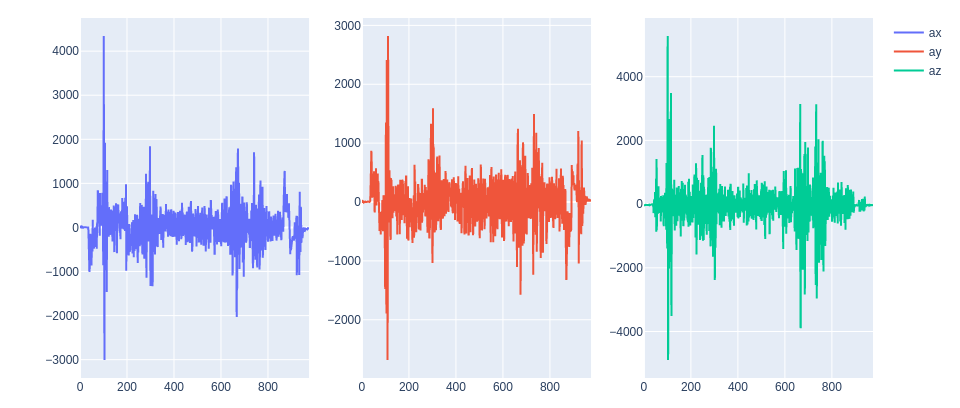
\includegraphics[scale=0.5]{img/DATA9.png}
    \caption{Données accélérométriques enregistrées sur le robot Scout 2.0 avec le dispositif Arduino}
    \label{bump_1}
\end{figure}

% \noindent
% \begin{minipage}[!hc]{0.12\textwidth}
%    \textbf{Remark}
% \end{minipage}
% \vrule\enskip\vrule\quad\begin{minipage}{\dimexpr 0.87\textwidth-0.8pt-1.5em}
% The sampling frequency (i.e. horizontal granularity) is defined by the Arduino program as: \(f = \frac{1}{10 \times 10^{-3}}\) which correspond to a delay of 10 ms between two measures.\\
% It is important to pay attention to the vertical scale of each graph.
% \end{minipage}

En parallèle, nous avions aussi débuté le développement d'une application Android pour permettre d'enregistrer des données plus précises et de façon plus efficace.